\section{PCB Design}\label{sec:PCB}
\todo[color=c05c,inline]{testing the colors}

To be able to test the proposed topology,
a Printed Circuit Board (PCB) had to be made.
We started out designing a simple two stage layout,
and ended up manufacturing a three stage version.

\subsection{Two Stage PCB}
To get familiar with designing power electronics PCBs,
we started out designing a two stage version of the proposed topology.
Because we already had some familiarities with EAGLE from previous projects,
we used EAGLE for the first design attempts.
The finished design can be seen in Figure \ref{fig:2nxeagle}.

\begin{figure}[H]
	\begin{center}
	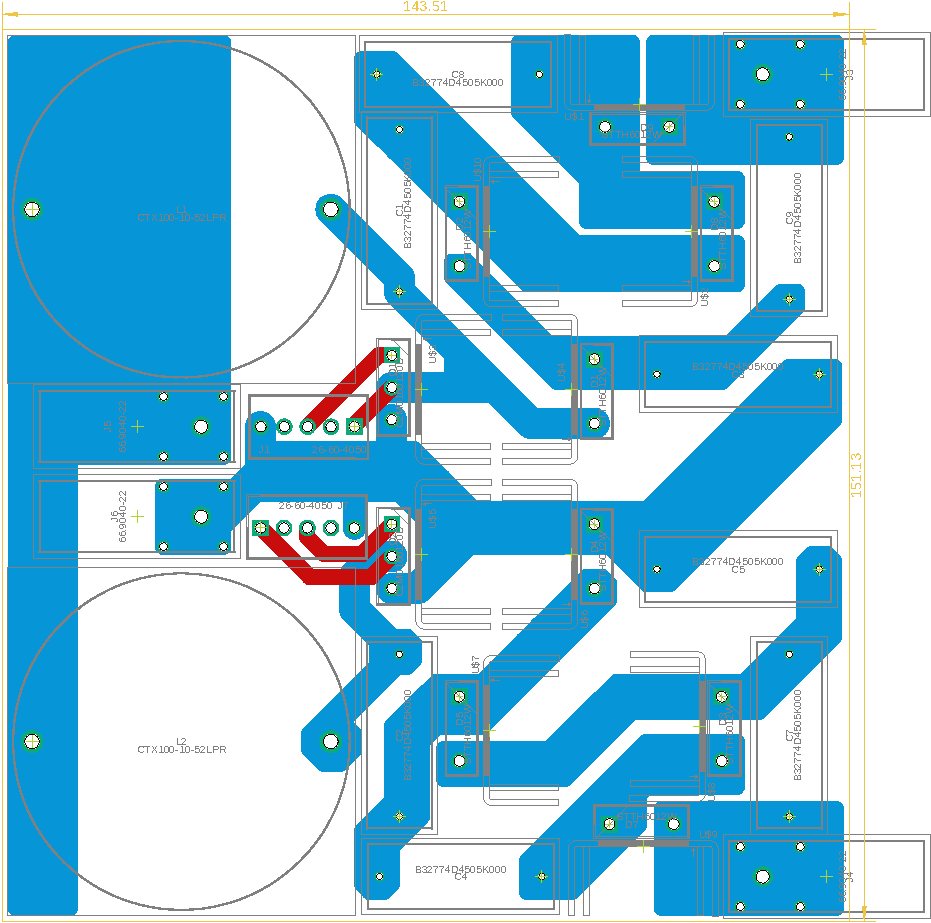
\includegraphics[width=0.6\textwidth]{figures/05cPCBdesign/2NX_interleaved_boost_converter_EAGLE_BY_DANIEL.pdf}
	\end{center}
	\caption{PCB Layout for a two stage 2NX Interleaved Boost Converter}
	\label{fig:2nxeagle}
\end{figure}

The red traces are logical signals,
located on the top layer of the PCB,
blue are power traces located on the bottom layer.
The power traces can be observed to be broader than the logic,
and were drawn as polygons,
to use the biggest available surface area.
The logical signals are designed to be as short as possible
and to be located as far from the power traces as possible,
to minimize interference.

Precautions were made in respect to the method of manufacturing,
because acute angles between two legs of a trace can lead to cracks in the trace when etching.
To prevent this from happening,
more copper was added in the areas in question to create obtuse angles.
A detailed view of this can be seen in Figure \ref{fig:2nxeagledetail}.
\begin{figure}[H]
	\begin{center}
	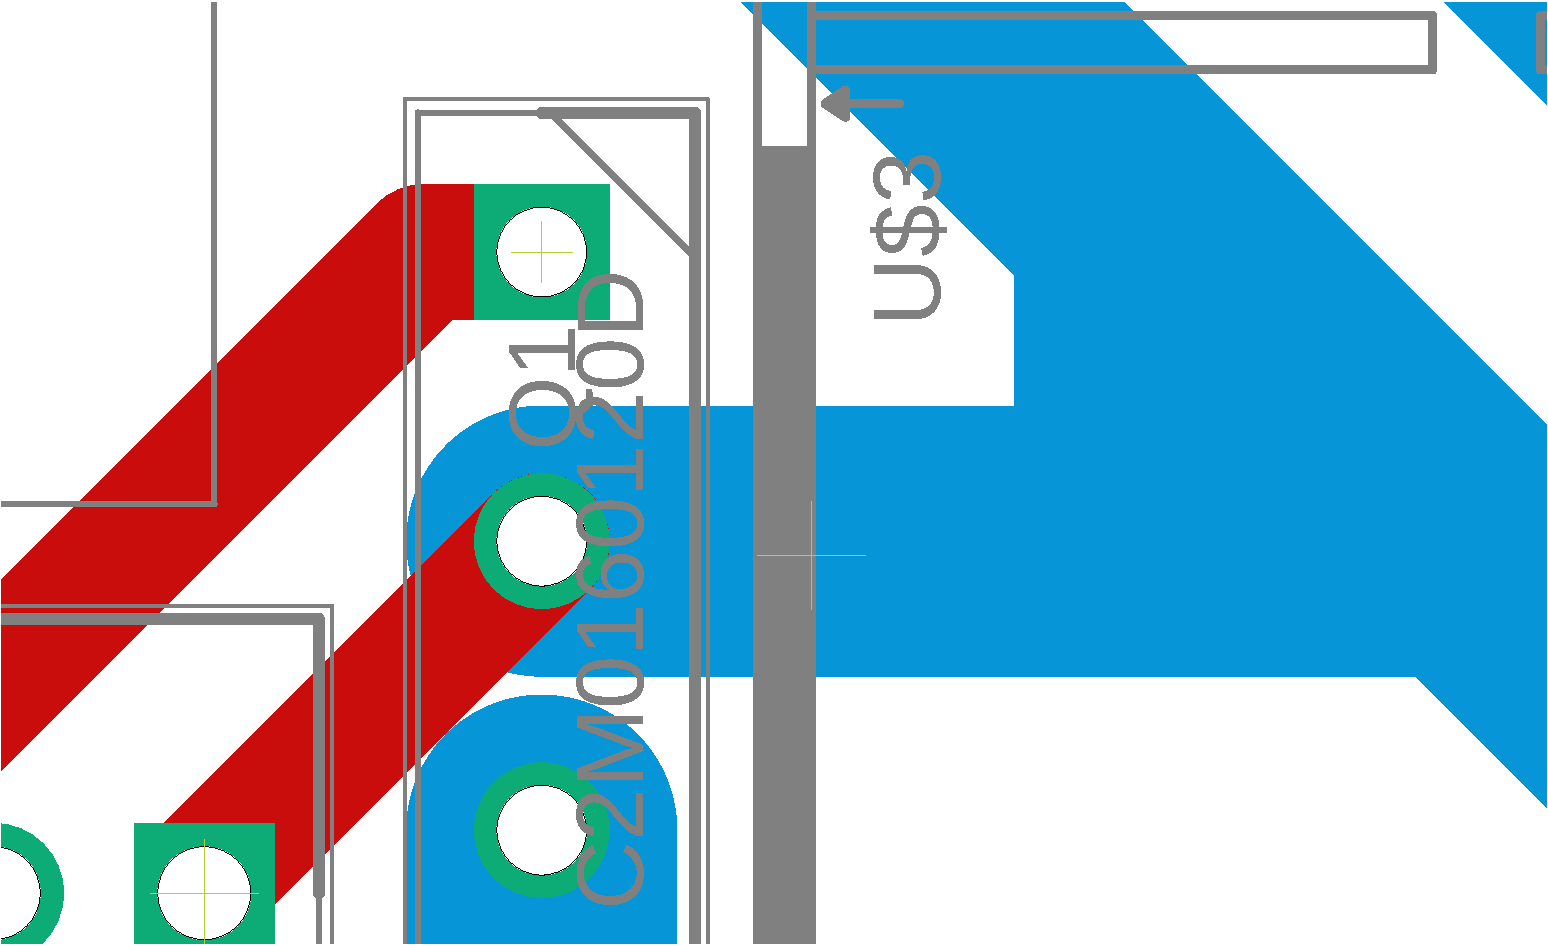
\includegraphics[width=0.6\textwidth]{figures/05cPCBdesign/2NX_interleaved_boost_converter_EAGLE_BY_DANIEL_DETAIL.pdf}
	\end{center}
	\caption{Detailed view of copper traces with obtuse angles}
	\label{fig:2nxeagledetail}
\end{figure}

\subsection{Three Stage PCB}\label{sub:3sPCB}
For the actual testing,
we decided on a three stage variant with our supervisor.
The PCB was again designed by us,
using feedback on the first design.
The power and logic traces are now on the same layer,
as it is not necessary to separate them as much.
The tracks generally are wider
and the spacing between is consistently kept at 2 mm.
The final PCB layout can be seen in Figure \ref{fig:multi2nxEAGLE}.

\begin{figure}[H]
	\begin{center}
	\includegraphics[height=0.6\textwidth,angle=270]{"figures/05cPCBdesign/FULL_3level_2NX_interleaved_boost_converter"}
	\end{center}
	\caption{PCB Layout for a multi stage 2NX Interleaved Boost Converter}
	\label{fig:multi2nxEAGLE}
\end{figure}

The inductors and capacitors are different to the previous design,
because the new design reflects the components available to us.
To be able to connect the board to power and measurements,
banana plugs were suggested by our supervisor.

The inductor is not connected directly by soldering,
but through jumper cables.
This allows for easier access to the core and to fine tune the windings after testing.
This also makes measuring of voltage and current easier.

A detailed view showing the connectors for the top inductor can be seen in Figure \ref{fig:multi2nxDetail}.\\
The banana plugs for connecting the inductor are shown in red.

\begin{figure}[H]
	\begin{center}
	\includegraphics[width=0.6\textwidth]{"figures/05cPCBdesign/DETAiL_3level_2NX_interleaved_boost_converter"}
	\end{center}
	\caption{Detailed view of the inductor connection}
	\label{fig:multi2nxDetail}
\end{figure}
